\chapter{Rotas dos drones}
\label{ch:identificador}
  
O uso de drones da nossa empresa tem como objetivo tornar as entregas mais rápidas no menor tempo possível e ter um aumento nos números de entregas com uma estimativa da média de 336 mil entregas por bairro sendo utilizado no total em nove bairros mas incrementamos em dois bairros como um exemplo de como seria.\\
Os drones em si teriam uma tecnologia de cálculo de rotas com uma análise rápida para obter uma certa agilidade, cada ponto de apoio teria uma equipe totalmente treinada com esse tipo de serviço além de certificados comprovando que são capazes do manuseio de drones com total eficiência.\\
Uma das maneiras que poderiam ser solicitadas às entregas seria da seguinte forma: os nossos serviços seriam solicitados, o drone iria levar a encomenda até a base para completar a entrega e o entregador ‘’motoboy’’ iria só a finalizar.

 \section{Bela Vista}

Bela Vista é um bairro relativamente pequeno quando o assunto é acrescentar drones para entrega, tendo um raio aproximadamente 2,6 km² com uma população de cerca de 70 mil habitantes. Esse bairro por si só tem uma certa fama pois é conhecido como o bairro do Bixiga, sendo uma das suas lendárias atrações paulistas além de teatros e do Museu de Arte de São Paulo.\\
Na imagem abaixo mostra que nesse bairro que não é muito grande, nos instalaremos uma única base de apoio tendo nela 10 drones disponíveis, monitorados por uma equipe especializada com certificado para o uso de drones com um regulamento de manter uma certa distância das pessoas pelo menos 30 metros e com a altura do voo do drone de 50 metros seguindo as mesmas rotas das nossas motos porém com mais rapidez. 

\begin{figure} [!ht]
   { \centering
   \caption{Rota do drone no bairro Bela Vista}
    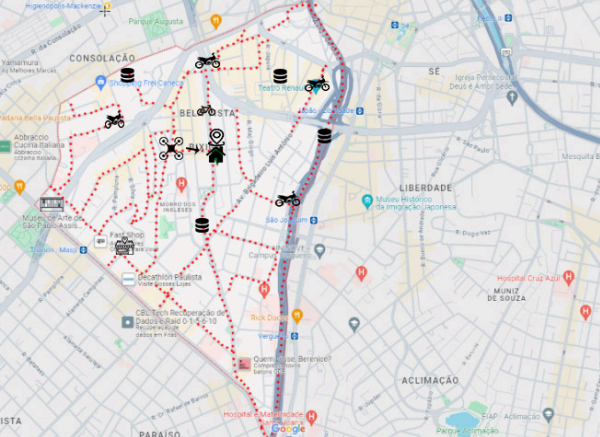
\includegraphics[width=0.5\linewidth]{figuras/rota bela vista.png}
    \label{fig:enter-label}
    \fonte{https://maps.app.goo.gl/8MuL8D5QTETv6svq8}
    }
\end{figure}

 \section{Santa Cecília}

 O Bairro de Santa Cecília, localizado na zona central do município de São Paulo, abrange uma área de aproximadamente 2,1 km². É um espaço onde o tradicional e o moderno convivem em harmonia, oferecendo uma rica experiência cultural e culinária aos seus moradores e visitantes, tendo uma população aproximadamente
de 15 mil habitantes. Santa Cecília possui alguns pontos turísticos como: Paróquia de Santa Cecília, Praça Frederico Arbegaus, Estátua do Gaúcho entre outras, além de sua própria história, contendo várias crises e mudanças e contendo seu renascimento
como um novo bairro.\\
Logo abaixo temos uma imagem de como seria a implementação dos drones nesse bairro escolhido, seguindo todas as normas e regulamentações para o uso de drones.

\begin{figure} [!ht]
    {\centering
    \caption{Rota do drone no bairro Santa Cecília}
    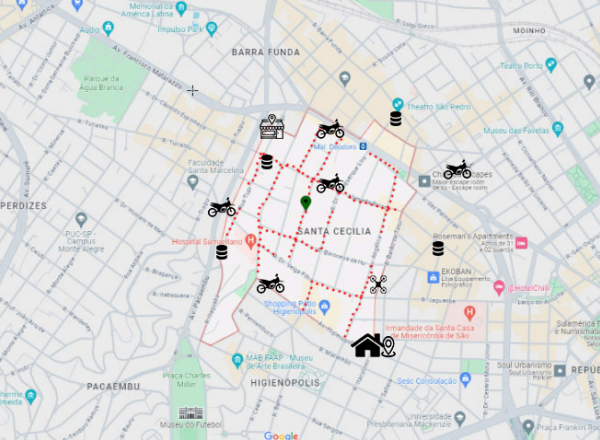
\includegraphics[width=0.9\linewidth]{figuras/rota santa cecilia.png}
    \label{fig:enter-label}
    \fonte{https://maps.app.goo.gl/YwaVA79U32ioDPiz8}
    }
\end{figure}

